\documentclass[14pt]{article}
\usepackage[utf8]{inputenc}
\usepackage{graphicx}
\usepackage{siunitx}
\usepackage[table]{xcolor}
\usepackage{amsmath}
\usepackage{geometry}
\usepackage{setspace}
\usepackage{enumitem}
\usepackage{titlesec}

\geometry{a4paper,
 total={170mm,257mm},
 left=30mm,
 right=30mm,
 bottom=40mm,
 top=44mm}

\sisetup{
    group-separator={,},
    group-minimum-digits=3,
    round-mode=places,
    round-precision=2,
    table-format=3.2
}

% header/footer images
\usepackage{eso-pic}
{% raw %}
\IfFileExists{logo.JPG}{%
  \AddToShipoutPictureBG{%
    \AtPageUpperLeft{\raisebox{-\height}{
\includegraphics[width=\paperwidth]{logo.JPG}}}
  }
  \AddToShipoutPictureFG{%
    \AtPageLowerCenter{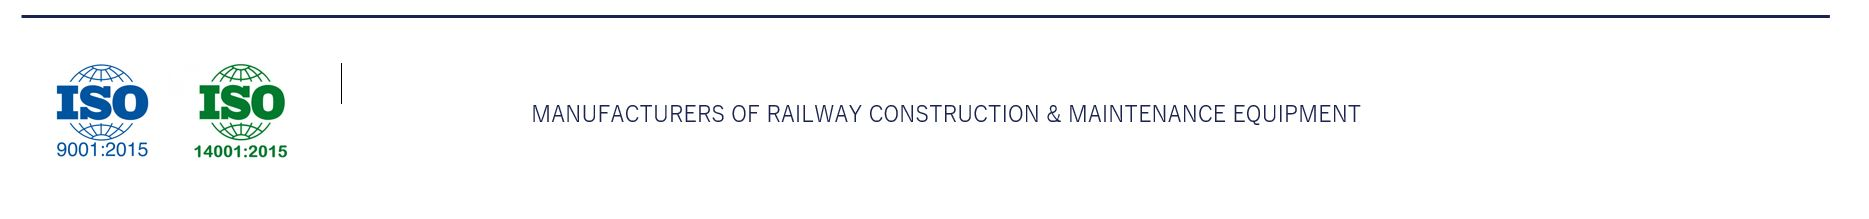
\includegraphics[height=2.3cm]{logo-1.JPG}}
  }
}
{% endraw %}

\usepackage{fancyhdr}
\pagestyle{fancy}
\fancyhf{}
\renewcommand{\headrulewidth}{0pt}
\fancyhead[R]{\fcolorbox{black}{white}{\small\texttt{ {{ data.doc_no | default('PEW57-003-00') }} }}}
\fancyfoot[C]{\thepage}

\begin{document}
\vspace*{1cm}

\begin{center}
{\LARGE\color{black}\textbf{Calculation of Spline Parameters for Gear Box\\
shaft and Half Gear Coupling}}\\[1ex]
\fcolorbox{black}{white}{\small\texttt{Doc NO. - {{ data.doc_no | default('PEW57-003-00') }}}}\\[2ex]
{\color{black}Made By: {{ data.made_by | default('Gauransh Kaushik') }}}\\
{\color{black}Checked By: {{ data.checked_by | default('Jasbir Singh') }}}\\
{\color{black}Approved By: {{ data.approved_by | default('Madhav Arora') }}}\\[1ex]
{{ data.doc_date | default("November 19, 2024") }}
\end{center}

\thispagestyle{fancy}

%% ─── 1. Introduction ────────────────────────────────────────────────────────
\section*{1\quad Introduction}
This document outlines the calculations involved in determining key parameters of splines used
to transmit torque in mechanical systems. These parameters include the pitch diameter, base
diameter, tooth thickness, fillet radius, torque capacity, and shear stress.

%% ─── 2. Spline Specifications ───────────────────────────────────────────────
\section*{2\quad Spline Specifications}
\begin{itemize}
  \item Number of teeth ($Z$)
  \item Diametral pitch ($P$) (teeth per unit diameter)
  \item Pressure angle ($\phi$)
  \item Material properties
\end{itemize}

%% ─── 3. Calculations ────────────────────────────────────────────────────────
\section*{3\quad Calculations}

\subsection*{3.1\quad Pitch Diameter (D)}
The pitch diameter is calculated using the formula:
\[ D = \frac{Z}{P} \]
where $Z$ is the number of teeth and $P$ is the diametral pitch.

\subsection*{3.2\quad Base Diameter ($D_b$)}
The base diameter, necessary for the involute profile, is calculated as:
\[ D_b = D\cos(\phi) \]
where $D$ is the pitch diameter and $\phi$ is the pressure angle.

\subsection*{3.3\quad Tooth Thickness (t)}
Tooth thickness at the pitch diameter:
\[ t = \frac{\pi}{2P} \]
where $P$ is the diametral pitch.

\subsection*{3.4\quad Fillet Radius (r)}
The fillet radius is determined based on the spline standard and ensures the teeth are not prone
to breakage.

\subsection*{3.5\quad Torque Capacity (T)}
Calculated by:
\[ T = \frac{D \times H \times L \times Z \times \tau_a}{2} \]
where $D$ is the pitch diameter, $H$ is the height of teeth, $L$ is the length of engagement,
$Z$ is the number of teeth, and $\tau_a$ is the allowable shear stress.

\subsection*{3.6\quad Shear Stress ($\tau$)}
Shear stress in the spline teeth:
\[ \tau = \frac{2 \times T}{D \times L \times Z \times H} \]
where $T$ is the torque transmitted, $D$ is the pitch diameter, $L$ is the length of engagement,
and $Z$ is the number of teeth.

%% ─── 4. Example ─────────────────────────────────────────────────────────────
\section*{4\quad Example}
To illustrate the calculation, consider the input values used in this report. The following
results are obtained by applying the formulas of Section~3 to the measured data.

%% 4.0.1 Pitch Diameter
\subsection*{4.0.1\quad Pitch Diameter (D)}
Given that the pitch diameter $D$ is:
\[ D = \frac{Z}{P} = \frac{ {{ result.Z | round(2) }} }{ {{ result.P | round(2) }} } = {{ result.D | round(2) }}\ \mathrm{mm} \]

%% 4.0.2 Base Diameter
\subsection*{4.0.2\quad Base Diameter ($D_b$)}
To calculate the base diameter $D_b$, we need the pressure angle $\phi$.
\[ D_b = D\cos(\phi) \]
\[ \phi = {{ data.pressure_angle | default(data.pressure_angle_deg) | default(0) }}^\circ \]
\[ D_b = {{ result.D | round(2) }}\cos({{ data.pressure_angle | default(data.pressure_angle_deg) | default(0) }}) = {{ result.base_diameter | round(2) }}\ \mathrm{mm} \]

%% 4.0.3 Tooth Thickness
\subsection*{4.0.3\quad Tooth Thickness (t)}
To calculate the tooth thickness at the pitch diameter, we need the diametral pitch $P$,
which is calculated as:
\[ P = \frac{Z}{D} \]
Substituting $Z={{ result.Z | int }}$ and $D={{ result.D | round(2) }}$ mm:
\[ P = \frac{ {{ result.Z | int }} }{ {{ result.D | round(2) }} } = {{ result.P | round(2) }}\ \text{teeth/mm} \]
Now, using the formula for tooth thickness:
\[ t = \frac{\pi}{2P} = \frac{\pi}{2 \times {{ result.P | round(2) }}} = {{ result.tooth_thickness | round(2) }}\ \mathrm{mm} \]

%% 4.0.4 Torque Capacity
\subsection*{4.0.4\quad Torque Capacity (T)}
The torque capacity is calculated using the formula:
\[ T = \frac{D \times H \times L \times Z \times \tau_a}{2} \]
Where:
\begin{itemize}[leftmargin=*]
  \item $D = {{ result.D | round(2) }}\ \mathrm{mm}$
  \item $H = (OD - ID)/2 = {{ result.H | round(2) }}\ \mathrm{mm}$
  \item $L = {{ data.length_engagement }}\ \mathrm{mm}$
  \item $Z = {{ result.Z | int }}$
  \item For {{ data.material_type | default('given material') }}:\\
        $\tau_a = 0.577 \times S_{yt} = 0.577 \times {{ result.yield_strength | round(2) }}\ \mathrm{MPa} = {{ result.allowable_shear | round(2) }}\ \mathrm{MPa}$
\end{itemize}
Substituting these values:
\[ T = \frac{ {{ result.D | round(2) }} \times {{ result.H | round(2) }} \times {{ data.length_engagement }} \times {{ result.Z | int }} \times {{ result.allowable_shear | round(2) }} }{2} \]
\[ \boxed{T = {{ result.torque_capacity | round(2) }}\ \mathrm{kNm}} \]

%% 4.0.5 Working Torque per Wheel
\subsection*{4.0.5\quad Working Torque per Wheel (T1)}
Working conditions:
\begin{itemize}[leftmargin=*]
  \item Locomotive Weight: ${{ data.loco_weight }}$ tons
  \item Number of Axles: ${{ data.number_axles }}$
  \item Number of wheels per axle: ${{ data.wheels_per_axle }}$
  \item Speed: ${{ data.speed }}$ km/h
  \item Wheel Diameter: ${{ data.wheel_diameter }}$ m
  \item Coefficient of Friction: ${{ data.friction_coeff }}$
\end{itemize}

\noindent\textbf{Rolling Resistance:}
\[ \text{Rolling Resistance} = (A + B \times \text{Speed} + C \times \text{Speed}^2) \times \text{Loco. Weight} \times g \]
\[ A = 0.647 + \frac{13.17}{\text{Loco. Weight} / \text{Axles}} = 0.647 + \frac{13.17}{ {{ data.loco_weight }} / {{ data.number_axles }} } = {{ result.A | round(2) }} \]
\[ B = 0.00933 \]
\[ C = \frac{0.057}{\text{Loco. Weight}} = \frac{0.057}{ {{ data.loco_weight }} } = {{ result.C | round(2) }} \]
\[ \text{Rolling Resistance} = {{ (result.rolling_resistance_n / 1000) | round(2) }}\ \mathrm{kN} \]

\noindent\textbf{Starting Resistance:}
\[ \text{Starting Resistance} = 6 \times \text{Loco. Weight} \times g = {{ (result.starting_resistance_n / 1000) | round(2) }}\ \mathrm{kN} \]

\noindent\textbf{Total Resistance:}\\
Total Resistance = Rolling Resistance $+$ Gradient Resistance $+$ Curvature Resistance $+$ Starting Resistance\\[0.5ex]
Total Resistance $= {{ (result.total_resistance_n / 1000) | round(2) }}\ \mathrm{kN}$
\quad $\because$ Gradient Resistance and Curvature Resistance are taken as zero

\[ T_1 = \frac{\text{Total Resistance} \times 1000 \times \text{Wheel Radius}}{\text{Number of Wheels}} = {{ result.working_torque_wheel | round(2) }}\ \mathrm{Nm} \]

%% 4.0.6 Working Shear Stress
\subsection*{4.0.6\quad Working Shear Stress ($\tau$)}
For the shear stress calculation, the formula is:
\[ \tau = \frac{2 \times T_1}{D \times L \times Z \times H} \]
Where:
\begin{itemize}[leftmargin=*]
  \item $D = {{ result.D | round(2) }}\ \mathrm{mm}$
  \item $H = {{ result.H | round(2) }}\ \mathrm{mm}$
  \item $L = {{ data.length_engagement }}\ \mathrm{mm}$
  \item $Z = {{ result.Z | int }}$
  \item $T_1 = {{ result.working_torque_wheel | round(2) }}\ \mathrm{Nm}$
\end{itemize}
Substituting:
\[ \tau = \frac{2 \times {{ result.working_torque_wheel | round(2) }} \times 10^3}{ {{ result.D | round(2) }} \times {{ data.length_engagement }} \times {{ result.Z | int }} \times {{ result.H | round(2) }} } = {{ result.shear_stress_wheel | round(2) }}\ \mathrm{MPa} \]

\noindent\textbf{Factor of Safety (FOS):}
\[ \text{FOS} = \frac{\tau_a}{\tau} = \frac{ {{ result.allowable_shear | round(2) }}\ \mathrm{MPa} }{ {{ result.shear_stress_wheel | round(2) }}\ \mathrm{MPa} } = {{ result.safety_factor | round(2) }} \]

%% 4.0.7 Summary
\subsection*{4.0.7\quad Summary of Results}
\begin{itemize}[leftmargin=*]
  \item Tooth Thickness ($t$): ${{ result.tooth_thickness | round(2) }}\ \mathrm{mm}$
  \item Torque Capacity ($T$): ${{ result.torque_capacity | round(2) }}\ \mathrm{kNm}$
  \item Working Torque per Wheel ($T_1$): ${{ result.working_torque_wheel | round(2) }}\ \mathrm{Nm}$
  \item Working Shear Stress ($\tau$): ${{ result.shear_stress_wheel | round(2) }}\ \mathrm{MPa}$
  \item Allowable Shear Stress ($\tau_a$): ${{ result.allowable_shear | round(2) }}\ \mathrm{MPa}$
  \item FOS at working torque: ${{ result.safety_factor | round(2) }}$
\end{itemize}

%% ─── 5. Conclusion ──────────────────────────────────────────────────────────
\section*{5\quad Conclusion}
This document provides the theoretical and practical calculations necessary for designing splines
capable of transmitting torque effectively in mechanical systems.

\vspace*{1cm}
{\color{black}\rule{\linewidth}{2pt}}
\end{document}
